\newpage
\subsection{Caso d'uso UC2: Registrazione}
\begin{center}
	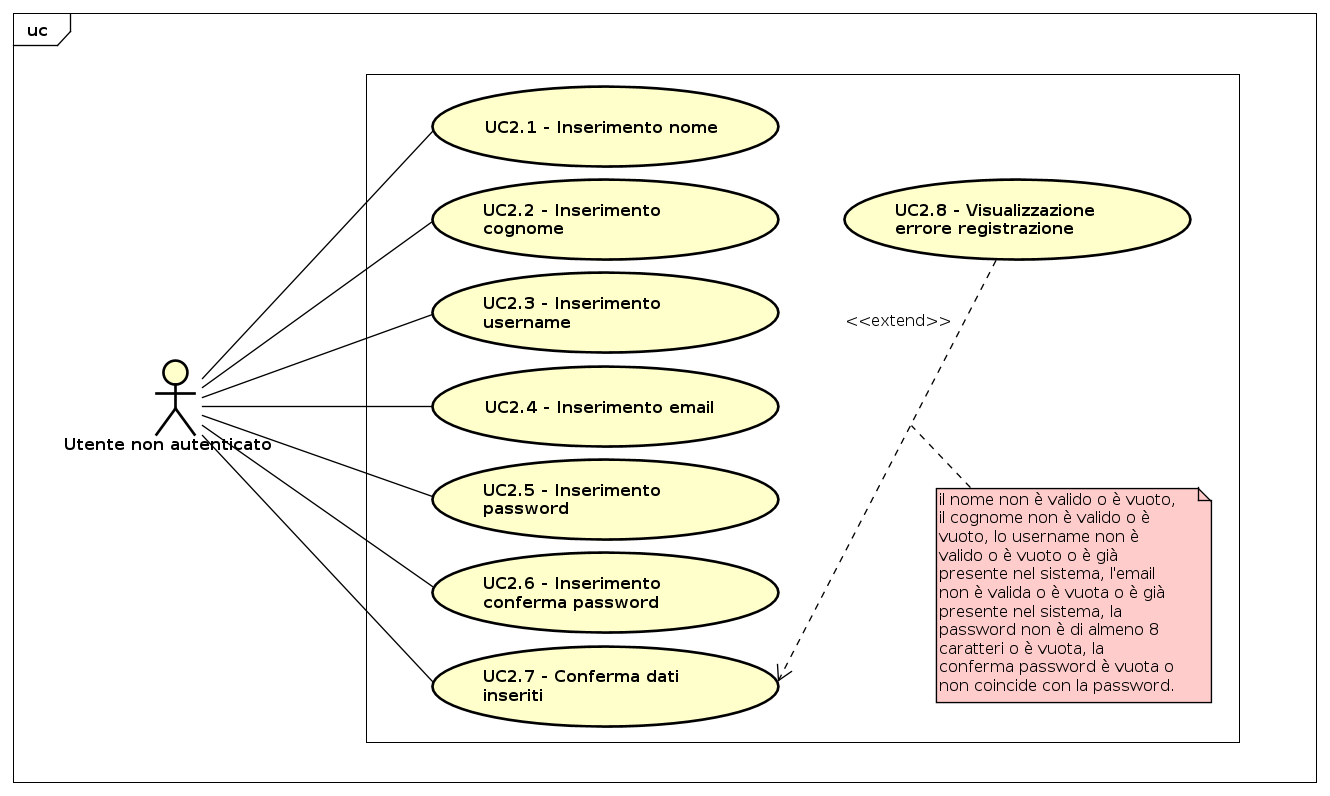
\includegraphics[scale=0.5]{UML/UC2.png}
\end{center}
\begin{itemize}
\item \textbf{Attori}: utente non autenticato;
\item \textbf{Descrizione}: per poter usufruire dei servizi forniti dalla piattaforma, l'attore deve registrarsi inserendo email e password;
\item \textbf{Precondizione}: il sistema è avviato e mostra la pagina iniziale;
\item \textbf{Postcondizione}: il sistema ha registrato l'attore.
\item \textbf{Scenario principale}:
	\begin{enumerate}
	\item L'attore inserisce il proprio nome (UC2.1);
	\item L'attore inserisce il proprio cognome (UC2.2);
	\item L'attore sceglie uno username (UC2.3);
	\item L'attore inserisce l'email (UC2.4);
	\item L'attore inserisce la password (UC2.5);
	\item L'attore inserisce una seconda volta la password (UC2.6);
	\item L'attore conferma i dati inseriti (UC2.7).
	\end{enumerate}
\item \textbf{Estensione}: l'attore visualizza un messaggio di errore (UC2.8).
\item \textbf{Scenario alternativo}: possono verificarsi uno o più dei seguenti scenari:
	\begin{itemize}
	\item[-] Il nome inserito non è valido oppure è vuoto;
	\item[-] Il cognome inserito non è valido oppure è vuoto;
	\item[-] Lo username inserito non è valido oppure è vuoto;
	\item[-] Lo username inserito è già presente nel sistema;
	\item[-] L'email inserita non è valida oppure è vuota;
	\item[-] L'email inserita è già presente nel sistema;
	\item[-] La password inserita è vuota oppure non è di almeno 8 caratteri;
	\item[-] La password e la conferma password non coincidono.
	\end{itemize}
In tal caso il sistema ritorna allo stato precedente l'inserimento dei dati visualizzando un messaggio di errore;
\end{itemize}

\subsubsection{Caso d'uso UC2.1: Inserimento nome}
\begin{itemize}
\item \textbf{Attori}: utente non autenticato;
\item \textbf{Descrizione}: l'attore può inserire il proprio nome per potersi registrare;
\item \textbf{Precondizione}: il sistema presenta all'attore lo spazio destinato a questa operazione;
\item \textbf{Postcondizione}: il nome è stato inserito.
\item \textbf{Scenario principale}: l'attore inserisce il proprio nome per potersi registrare;
\end{itemize}

\subsubsection{Caso d'uso UC2.2: Inserimento cognome}
\begin{itemize}
\item \textbf{Attori}: utente non autenticato;
\item \textbf{Descrizione}: l'attore può inserire il proprio cognome per potersi registrare;
\item \textbf{Precondizione}: il sistema presenta all'attore lo spazio destinato a questa operazione;
\item \textbf{Postcondizione}: il cognome è stato inserito.
\item \textbf{Scenario principale}: l'attore inserisce il proprio cognome per potersi registrare;
\end{itemize}

\subsubsection{Caso d'uso UC2.3: Inserimento username}
\begin{itemize}
\item \textbf{Attori}: utente non autenticato;
\item \textbf{Descrizione}: l'attore può inserire il proprio username per potersi registrare;
\item \textbf{Precondizione}: il sistema presenta all'attore lo spazio destinato a questa operazione;
\item \textbf{Postcondizione}: lo username è stato inserito.
\item \textbf{Scenario principale}: l'attore inserisce il proprio username per potersi registrare;
\end{itemize}

\subsubsection{Caso d'uso UC2.4: Inserimento email}
\begin{itemize}
\item \textbf{Attori}: utente non autenticato;
\item \textbf{Descrizione}: l'attore può inserire il proprio indirizzo email per potersi registrare;
\item \textbf{Precondizione}: il sistema presenta all'attore lo spazio destinato a questa operazione;
\item \textbf{Postcondizione}: l'email è stata inserita.
\item \textbf{Scenario principale}: l'attore inserisce il proprio indirizzo email per potersi registrare; 
\end{itemize}

\subsubsection{Caso d'uso UC2.5: Inserimento password}
\begin{itemize}
\item \textbf{Attori}: utente non autenticato;
\item \textbf{Descrizione}: l'attore può inserire una password a sua scelta per potersi registrare;
\item \textbf{Precondizione}: il sistema presenta all'attore lo spazio destinato a questa operazione;
\item \textbf{Postcondizione}: la password è stata inserita.
\item \textbf{Scenario principale}: l'attore inserisce una password a sua scelta per potersi registrare;
\end{itemize}

\subsubsection{Caso d'uso UC2.6: Inserimento conferma password}
\begin{itemize}
\item \textbf{Attori}: utente non autenticato;
\item \textbf{Descrizione}: l'attore può inserire nuovamente la password scelta;
\item \textbf{Precondizione}: il sistema presenta all'attore lo spazio destinato a questa operazione;
\item \textbf{Postcondizione}: la conferma della password è stata inserita.
\item \textbf{Scenario principale}: l'attore inserisce nuovamente la password scelta;
\end{itemize}

\subsubsection{Caso d'uso UC2.7: Conferma registrazione}
\begin{itemize}
\item \textbf{Attori}: utente non autenticato;
\item \textbf{Descrizione}: l'attore può confermare i dati inseriti;
\item \textbf{Precondizione}: il sistema presenta all'attore lo spazio destinato a questa operazione;
\item \textbf{Postcondizione}: il sistema ha ricevuto i dati per la registrazione.
\item \textbf{Scenario principale}: l'attore conferma i dati inseriti;
\end{itemize}

\subsubsection{Caso d'uso UC2.8: Visualizzazione errore registrazione}
\begin{itemize}
\item \textbf{Attori}: utente non autenticato;
\item \textbf{Descrizione}: l'attore può visualizzare un messaggio d'errore nel caso si fossero verificati uno o più scenari alternativi;
\item \textbf{Precondizione}: il sistema ha ricevuto dei dati errati per la registrazione;
\item \textbf{Postcondizione}: il sistema mostra un messaggio di errore.
\item \textbf{Scenario principale}: l'attore visualizza un messaggio d'errore nel caso si fossero verificati uno o più scenari alternativi;
\end{itemize}
